\documentclass{article}
\usepackage{amsmath}
\usepackage{amsthm}
\usepackage{biblatex}
\usepackage{graphicx}
\usepackage{hyperref}
\usepackage{cleveref}

\theoremstyle{plain}
\newtheorem{theorem}{Theorem}[section]
\newtheorem{corollary}{Corollary}[section]
\newtheorem{lemma}{Lemma}[section]
\newtheorem{proposition}{Proposition}[section]

\theoremstyle{definition}
\newtheorem{definition}{Definition}[section]
\newtheorem{example}{Example}

\theoremstyle{remark}
\newtheorem{remark}{Remark}[section]
\newtheorem{fact}[remark]{Fact}
\DeclareMathOperator{\aff}{aff}

\addbibresource{bibliography.bib}
\title{An example of how to use this plugin.}
\author{Matthew Scott}
\begin{document}
\maketitle
\begin{abstract}
This is the abstract. The abstract needs only be placed under an header named ``Abstract" in the longform note.
\end{abstract}
\section{Introduction}
\label{loc:body.introduction}
Most of the introduction is in another note. We embed its contents without creating a latex environment.
We \emph{have} \textbf{things} ``to" talk about. We can use latex macros: $\aff(T)$. We can reference markdown headers, which become references to latex sections: feel free to skip ahead to \Cref{loc:body.main_results}.

Results are referenced by linking notes: we will show that \Cref{loc:theorem_1.statement} holds by using \Cref{loc:lemma_1.statement}, \Cref{loc:lemma_2.statement}, \Cref{loc:other_small_lemmas.first_other_lemma} and \Cref{loc:other_small_lemmas.second_other_lemma}. We can state results through labelled embeds, as follows. 
\begin{lemma}
\label{loc:other_small_lemmas.second_other_lemma}
That the first lemma holds
\end{lemma}
Note that the above result was embedded into the note `introduction' which was itself embedded into the longform note, and this still produces a result that can be referenced from anywhere via wikilinks.
\section{Literature review}
\label{loc:body.literature_review}
We cite as follows: \cite{vershyninHighDimensionalProbabilityIntroduction2018}. A \emph{textcite} cand be also used: the book is by \textcite{vershyninHighDimensionalProbabilityIntroduction2018}. Specific results can be referenced: \cite[Example 5.4]{vershyninHighDimensionalProbabilityIntroduction2018}. Multi-citations are also supported: \cite{berkCoherenceParameterCharacterizing2022, berkModeladaptedFourierSampling2023}.

Alternatively, pandoc syntax also works, though you may want to set the default citation command to \emph{textcite} in the plugin settings. \cite{vershyninHighDimensionalProbabilityIntroduction2018}, \cite{vershyninHighDimensionalProbabilityIntroduction2018}, \cite[Example 2.1]{vershyninHighDimensionalProbabilityIntroduction2018}, \cite{berkCoherenceParameterCharacterizing2022, berkModeladaptedFourierSampling2023}, and then \cite{vershyninHighDimensionalProbabilityIntroduction2018}.
\section{Main results}
\label{loc:body.main_results}
Here is an equation that we can reference.
\begin{equation}
\label{eq:main}
1+1 = 2
\end{equation}
\begin{lemma}
\label{lem:explicit}
We reference the equation: \Cref{eq:main} and the result: \Cref{lem:explicit}.
\begin{align}
1+1 & = 1+3-2 \label{eq:aligned_eq:1}\\
& = 2 \label{eq:aligned_eq:2}
\end{align}
We can reference individual lines of an align environment: \Cref{eq:aligned_eq:1} and \Cref{eq:aligned_eq:2}.
\end{lemma}
The next result is in its own note. Embedding the `Statement' header as follows creates a latex environment.
\begin{theorem}
\label{loc:theorem_1.statement}
Indeed, $1+1  =  2$.
\end{theorem}
We can link to \hyperlink{loc:theorem_1.proof}{the proof} with a wikilink to the ``Proof" header.
The theorem environment is then referenced as \Cref{loc:theorem_1.statement}, or as \Cref{loc:theorem_1.statement}. To show \Cref{loc:theorem_1.statement}, we need the following two results.
\begin{lemma}
\label{loc:lemma_1.statement}
The first fact is that $10-9 = 1$
\end{lemma}
We defer \hyperlink{loc:lemma_1.proof}{the proof} to the appendix.
\begin{lemma}
\label{loc:other_small_lemmas.first_other_lemma}
A first additional lemma
\begin{equation*}
1+1 = 2
\end{equation*}
\end{lemma}
We can use lists. Also, results can live in the same note under different headers. We embedded two results from the same note: 
\begin{enumerate}
\item The first is \Cref{loc:other_small_lemmas.first_other_lemma}.
\item The other,\Cref{loc:other_small_lemmas.second_other_lemma}.
\end{enumerate}

There are also options for comments.
% This will become a comment in the latex export.
\section{Proofs}
\label{loc:body.proofs}
We are ready to prove our main result. We can embed proof environments from other notes. References to the correct results in the header of the proof are generated automatically.
\begin{proof}[\hypertarget{loc:theorem_1.proof}Proof of \Cref{loc:theorem_1.statement}]

For this we require another result.
\begin{proposition}
\label{loc:lemma_2.statement}
$1+4 = 5$
\end{proposition}
\begin{proof}[\hypertarget{loc:lemma_2.proof}Proof of \Cref{loc:lemma_2.statement}]

Left to the reader.
\end{proof}
and therefore we can finish the proof of \Cref{loc:theorem_1.statement}.
\end{proof}
\subsection{Sub-section for proofs}
\label{loc:body.proofs.sub:section_for_proofs}
There can be nested sections, which can be referenced via wikilinks from anywhere.
\section{Numerics}
\label{loc:body.numerics}
Behold! Figures with captions are supported! The relevant files will be copied over with the export.
\begin{figure}[h]
\centering
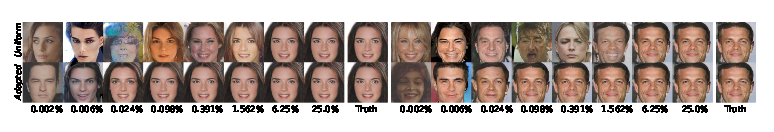
\includegraphics[width=0.5\textwidth]{Files/intro_comp_wlabel.pdf}
\caption{Captions of figures are specified in the display part of the figure's embed wikilink.\label{fig:intro_comp_wlabel.pdf}}
\end{figure}
We can reference the figures with a wikilink \Cref{fig:intro_comp_wlabel.pdf}.
\printbibliography
\appendix
\section{Appendix}
\begin{proof}[\hypertarget{loc:lemma_1.proof}Proof of \Cref{loc:lemma_1.statement}]

Ask chatgpt.
\end{proof}
\end{document}
